% Created by tikzDevice version 0.12.6 on 2025-02-12 15:30:51
% !TEX encoding = UTF-8 Unicode
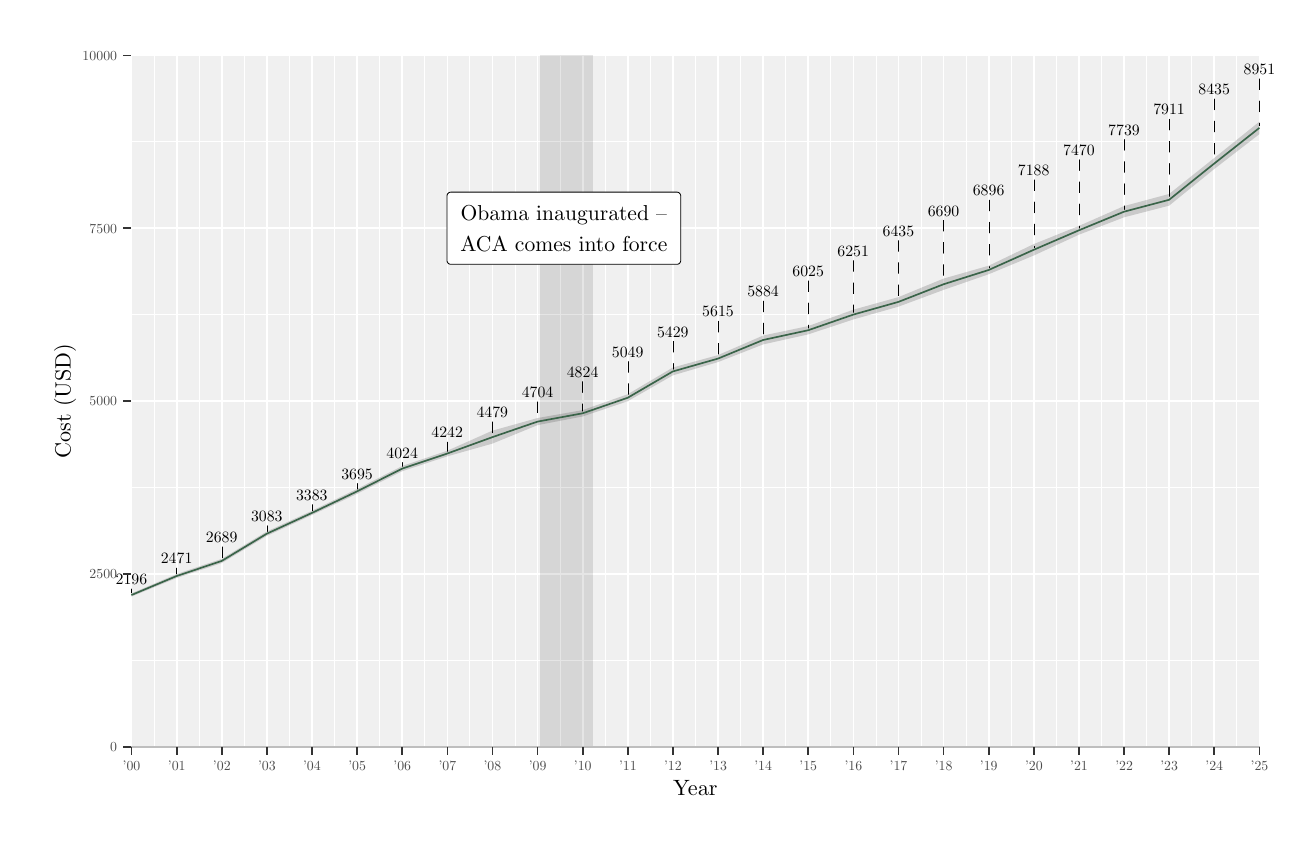
\begin{tikzpicture}[x=1pt,y=1pt]
\definecolor{fillColor}{RGB}{255,255,255}
\path[use as bounding box,fill=fillColor,fill opacity=0.00] (0,0) rectangle (455.30,289.08);
\begin{scope}
\path[clip] (  0.00,  0.00) rectangle (455.30,289.08);
\definecolor{drawColor}{RGB}{255,255,255}
\definecolor{fillColor}{RGB}{255,255,255}

\path[draw=drawColor,line width= 0.6pt,line join=round,line cap=round,fill=fillColor] ( -0.00,  0.00) rectangle (455.30,289.08);
\end{scope}
\begin{scope}
\path[clip] (  0.00,  0.00) rectangle (455.30,289.08);
\definecolor{fillColor}{gray}{0.94}

\path[fill=fillColor] ( 37.26, 29.18) rectangle (445.30,279.08);
\definecolor{drawColor}{RGB}{255,255,255}

\path[draw=drawColor,line width= 0.3pt,line join=round] ( 37.26, 60.42) --
	(445.30, 60.42);

\path[draw=drawColor,line width= 0.3pt,line join=round] ( 37.26,122.89) --
	(445.30,122.89);

\path[draw=drawColor,line width= 0.3pt,line join=round] ( 37.26,185.37) --
	(445.30,185.37);

\path[draw=drawColor,line width= 0.3pt,line join=round] ( 37.26,247.84) --
	(445.30,247.84);

\path[draw=drawColor,line width= 0.3pt,line join=round] ( 45.70, 29.18) --
	( 45.70,279.08);

\path[draw=drawColor,line width= 0.3pt,line join=round] ( 62.01, 29.18) --
	( 62.01,279.08);

\path[draw=drawColor,line width= 0.3pt,line join=round] ( 78.30, 29.18) --
	( 78.30,279.08);

\path[draw=drawColor,line width= 0.3pt,line join=round] ( 94.59, 29.18) --
	( 94.59,279.08);

\path[draw=drawColor,line width= 0.3pt,line join=round] (110.91, 29.18) --
	(110.91,279.08);

\path[draw=drawColor,line width= 0.3pt,line join=round] (127.22, 29.18) --
	(127.22,279.08);

\path[draw=drawColor,line width= 0.3pt,line join=round] (143.51, 29.18) --
	(143.51,279.08);

\path[draw=drawColor,line width= 0.3pt,line join=round] (159.80, 29.18) --
	(159.80,279.08);

\path[draw=drawColor,line width= 0.3pt,line join=round] (176.12, 29.18) --
	(176.12,279.08);

\path[draw=drawColor,line width= 0.3pt,line join=round] (192.43, 29.18) --
	(192.43,279.08);

\path[draw=drawColor,line width= 0.3pt,line join=round] (208.72, 29.18) --
	(208.72,279.08);

\path[draw=drawColor,line width= 0.3pt,line join=round] (225.01, 29.18) --
	(225.01,279.08);

\path[draw=drawColor,line width= 0.3pt,line join=round] (241.33, 29.18) --
	(241.33,279.08);

\path[draw=drawColor,line width= 0.3pt,line join=round] (257.64, 29.18) --
	(257.64,279.08);

\path[draw=drawColor,line width= 0.3pt,line join=round] (273.93, 29.18) --
	(273.93,279.08);

\path[draw=drawColor,line width= 0.3pt,line join=round] (290.22, 29.18) --
	(290.22,279.08);

\path[draw=drawColor,line width= 0.3pt,line join=round] (306.54, 29.18) --
	(306.54,279.08);

\path[draw=drawColor,line width= 0.3pt,line join=round] (322.85, 29.18) --
	(322.85,279.08);

\path[draw=drawColor,line width= 0.3pt,line join=round] (339.14, 29.18) --
	(339.14,279.08);

\path[draw=drawColor,line width= 0.3pt,line join=round] (355.43, 29.18) --
	(355.43,279.08);

\path[draw=drawColor,line width= 0.3pt,line join=round] (371.75, 29.18) --
	(371.75,279.08);

\path[draw=drawColor,line width= 0.3pt,line join=round] (388.06, 29.18) --
	(388.06,279.08);

\path[draw=drawColor,line width= 0.3pt,line join=round] (404.35, 29.18) --
	(404.35,279.08);

\path[draw=drawColor,line width= 0.3pt,line join=round] (420.64, 29.18) --
	(420.64,279.08);

\path[draw=drawColor,line width= 0.3pt,line join=round] (436.95, 29.18) --
	(436.95,279.08);

\path[draw=drawColor,line width= 0.6pt,line join=round] ( 37.26, 29.18) --
	(445.30, 29.18);

\path[draw=drawColor,line width= 0.6pt,line join=round] ( 37.26, 91.66) --
	(445.30, 91.66);

\path[draw=drawColor,line width= 0.6pt,line join=round] ( 37.26,154.13) --
	(445.30,154.13);

\path[draw=drawColor,line width= 0.6pt,line join=round] ( 37.26,216.61) --
	(445.30,216.61);

\path[draw=drawColor,line width= 0.6pt,line join=round] ( 37.26,279.08) --
	(445.30,279.08);

\path[draw=drawColor,line width= 0.6pt,line join=round] ( 37.53, 29.18) --
	( 37.53,279.08);

\path[draw=drawColor,line width= 0.6pt,line join=round] ( 53.87, 29.18) --
	( 53.87,279.08);

\path[draw=drawColor,line width= 0.6pt,line join=round] ( 70.16, 29.18) --
	( 70.16,279.08);

\path[draw=drawColor,line width= 0.6pt,line join=round] ( 86.45, 29.18) --
	( 86.45,279.08);

\path[draw=drawColor,line width= 0.6pt,line join=round] (102.74, 29.18) --
	(102.74,279.08);

\path[draw=drawColor,line width= 0.6pt,line join=round] (119.08, 29.18) --
	(119.08,279.08);

\path[draw=drawColor,line width= 0.6pt,line join=round] (135.37, 29.18) --
	(135.37,279.08);

\path[draw=drawColor,line width= 0.6pt,line join=round] (151.66, 29.18) --
	(151.66,279.08);

\path[draw=drawColor,line width= 0.6pt,line join=round] (167.95, 29.18) --
	(167.95,279.08);

\path[draw=drawColor,line width= 0.6pt,line join=round] (184.28, 29.18) --
	(184.28,279.08);

\path[draw=drawColor,line width= 0.6pt,line join=round] (200.58, 29.18) --
	(200.58,279.08);

\path[draw=drawColor,line width= 0.6pt,line join=round] (216.87, 29.18) --
	(216.87,279.08);

\path[draw=drawColor,line width= 0.6pt,line join=round] (233.16, 29.18) --
	(233.16,279.08);

\path[draw=drawColor,line width= 0.6pt,line join=round] (249.49, 29.18) --
	(249.49,279.08);

\path[draw=drawColor,line width= 0.6pt,line join=round] (265.79, 29.18) --
	(265.79,279.08);

\path[draw=drawColor,line width= 0.6pt,line join=round] (282.08, 29.18) --
	(282.08,279.08);

\path[draw=drawColor,line width= 0.6pt,line join=round] (298.37, 29.18) --
	(298.37,279.08);

\path[draw=drawColor,line width= 0.6pt,line join=round] (314.70, 29.18) --
	(314.70,279.08);

\path[draw=drawColor,line width= 0.6pt,line join=round] (330.99, 29.18) --
	(330.99,279.08);

\path[draw=drawColor,line width= 0.6pt,line join=round] (347.29, 29.18) --
	(347.29,279.08);

\path[draw=drawColor,line width= 0.6pt,line join=round] (363.58, 29.18) --
	(363.58,279.08);

\path[draw=drawColor,line width= 0.6pt,line join=round] (379.91, 29.18) --
	(379.91,279.08);

\path[draw=drawColor,line width= 0.6pt,line join=round] (396.20, 29.18) --
	(396.20,279.08);

\path[draw=drawColor,line width= 0.6pt,line join=round] (412.50, 29.18) --
	(412.50,279.08);

\path[draw=drawColor,line width= 0.6pt,line join=round] (428.79, 29.18) --
	(428.79,279.08);

\path[draw=drawColor,line width= 0.6pt,line join=round] (445.12, 29.18) --
	(445.12,279.08);
\definecolor{fillColor}{RGB}{190,190,190}

\path[fill=fillColor,fill opacity=0.01] (185.13, 29.18) rectangle (204.19,279.08);

\path[fill=fillColor,fill opacity=0.01] (185.13, 29.18) rectangle (204.19,279.08);

\path[fill=fillColor,fill opacity=0.01] (185.13, 29.18) rectangle (204.19,279.08);

\path[fill=fillColor,fill opacity=0.01] (185.13, 29.18) rectangle (204.19,279.08);

\path[fill=fillColor,fill opacity=0.01] (185.13, 29.18) rectangle (204.19,279.08);

\path[fill=fillColor,fill opacity=0.01] (185.13, 29.18) rectangle (204.19,279.08);

\path[fill=fillColor,fill opacity=0.01] (185.13, 29.18) rectangle (204.19,279.08);

\path[fill=fillColor,fill opacity=0.01] (185.13, 29.18) rectangle (204.19,279.08);

\path[fill=fillColor,fill opacity=0.01] (185.13, 29.18) rectangle (204.19,279.08);

\path[fill=fillColor,fill opacity=0.01] (185.13, 29.18) rectangle (204.19,279.08);

\path[fill=fillColor,fill opacity=0.01] (185.13, 29.18) rectangle (204.19,279.08);

\path[fill=fillColor,fill opacity=0.01] (185.13, 29.18) rectangle (204.19,279.08);

\path[fill=fillColor,fill opacity=0.01] (185.13, 29.18) rectangle (204.19,279.08);

\path[fill=fillColor,fill opacity=0.01] (185.13, 29.18) rectangle (204.19,279.08);

\path[fill=fillColor,fill opacity=0.01] (185.13, 29.18) rectangle (204.19,279.08);

\path[fill=fillColor,fill opacity=0.01] (185.13, 29.18) rectangle (204.19,279.08);

\path[fill=fillColor,fill opacity=0.01] (185.13, 29.18) rectangle (204.19,279.08);

\path[fill=fillColor,fill opacity=0.01] (185.13, 29.18) rectangle (204.19,279.08);

\path[fill=fillColor,fill opacity=0.01] (185.13, 29.18) rectangle (204.19,279.08);

\path[fill=fillColor,fill opacity=0.01] (185.13, 29.18) rectangle (204.19,279.08);

\path[fill=fillColor,fill opacity=0.01] (185.13, 29.18) rectangle (204.19,279.08);

\path[fill=fillColor,fill opacity=0.01] (185.13, 29.18) rectangle (204.19,279.08);

\path[fill=fillColor,fill opacity=0.01] (185.13, 29.18) rectangle (204.19,279.08);

\path[fill=fillColor,fill opacity=0.01] (185.13, 29.18) rectangle (204.19,279.08);

\path[fill=fillColor,fill opacity=0.01] (185.13, 29.18) rectangle (204.19,279.08);

\path[fill=fillColor,fill opacity=0.01] (185.13, 29.18) rectangle (204.19,279.08);
\definecolor{drawColor}{RGB}{190,190,190}

\path[draw=drawColor,line width= 0.6pt,line join=round] ( 37.26, 29.18) -- (445.30, 29.18);

\path[draw=drawColor,line width= 0.6pt,line join=round] (-451.52, 29.18) -- (-451.52,279.08);
\definecolor{drawColor}{RGB}{60,113,79}

\path[draw=drawColor,line width= 0.6pt,line join=round] ( 37.49, 84.06) --
	( 53.82, 90.93) --
	( 70.11, 96.38) --
	( 86.40,106.22) --
	(102.69,113.72) --
	(119.03,121.52) --
	(135.32,129.74) --
	(151.61,135.19) --
	(167.90,141.11) --
	(184.24,146.73) --
	(200.53,149.73) --
	(216.82,155.35) --
	(233.11,164.85) --
	(249.45,169.50) --
	(265.74,176.22) --
	(282.03,179.74) --
	(298.32,185.39) --
	(314.66,189.99) --
	(330.95,196.36) --
	(347.24,201.51) --
	(363.53,208.81) --
	(379.87,215.86) --
	(396.16,222.58) --
	(412.45,226.88) --
	(428.74,239.97) --
	(445.08,252.87);
\definecolor{fillColor}{RGB}{51,51,51}

\path[fill=fillColor,fill opacity=0.20] ( 37.49, 84.63) --
	( 53.82, 91.64) --
	( 70.11, 97.14) --
	( 86.40,107.02) --
	(102.69,114.48) --
	(119.03,122.41) --
	(135.32,130.68) --
	(151.61,136.20) --
	(167.90,143.45) --
	(184.24,148.02) --
	(200.53,150.88) --
	(216.82,156.62) --
	(233.11,166.27) --
	(249.45,170.76) --
	(265.74,177.83) --
	(282.03,181.25) --
	(298.32,187.16) --
	(314.66,191.71) --
	(330.95,198.41) --
	(347.24,203.05) --
	(363.53,210.87) --
	(379.87,217.44) --
	(396.16,224.61) --
	(412.45,228.99) --
	(428.74,241.96) --
	(445.08,255.12) --
	(445.08,250.61) --
	(428.74,237.98) --
	(412.45,224.76) --
	(396.16,220.55) --
	(379.87,214.27) --
	(363.53,206.74) --
	(347.24,199.97) --
	(330.95,194.32) --
	(314.66,188.27) --
	(298.32,183.63) --
	(282.03,178.24) --
	(265.74,174.61) --
	(249.45,168.24) --
	(233.11,163.43) --
	(216.82,154.09) --
	(200.53,148.58) --
	(184.24,145.45) --
	(167.90,138.77) --
	(151.61,134.17) --
	(135.32,128.80) --
	(119.03,120.63) --
	(102.69,112.97) --
	( 86.40,105.43) --
	( 70.11, 95.62) --
	( 53.82, 90.22) --
	( 37.49, 83.49) --
	cycle;

\path[] ( 37.49, 84.63) --
	( 53.82, 91.64) --
	( 70.11, 97.14) --
	( 86.40,107.02) --
	(102.69,114.48) --
	(119.03,122.41) --
	(135.32,130.68) --
	(151.61,136.20) --
	(167.90,143.45) --
	(184.24,148.02) --
	(200.53,150.88) --
	(216.82,156.62) --
	(233.11,166.27) --
	(249.45,170.76) --
	(265.74,177.83) --
	(282.03,181.25) --
	(298.32,187.16) --
	(314.66,191.71) --
	(330.95,198.41) --
	(347.24,203.05) --
	(363.53,210.87) --
	(379.87,217.44) --
	(396.16,224.61) --
	(412.45,228.99) --
	(428.74,241.96) --
	(445.08,255.12);

\path[] (445.08,250.61) --
	(428.74,237.98) --
	(412.45,224.76) --
	(396.16,220.55) --
	(379.87,214.27) --
	(363.53,206.74) --
	(347.24,199.97) --
	(330.95,194.32) --
	(314.66,188.27) --
	(298.32,183.63) --
	(282.03,178.24) --
	(265.74,174.61) --
	(249.45,168.24) --
	(233.11,163.43) --
	(216.82,154.09) --
	(200.53,148.58) --
	(184.24,145.45) --
	(167.90,138.77) --
	(151.61,134.17) --
	(135.32,128.80) --
	(119.03,120.63) --
	(102.69,112.97) --
	( 86.40,105.43) --
	( 70.11, 95.62) --
	( 53.82, 90.22) --
	( 37.49, 83.49);
\definecolor{drawColor}{RGB}{0,0,0}

\path[draw=drawColor,line width= 0.1pt,dash pattern=on 4pt off 4pt ,line join=round,line cap=round] ( 37.49, 86.30) -- ( 37.49, 84.80);

\path[draw=drawColor,line width= 0.1pt,dash pattern=on 4pt off 4pt ,line join=round,line cap=round] ( 53.82, 93.84) -- ( 53.82, 91.67);

\path[draw=drawColor,line width= 0.1pt,dash pattern=on 4pt off 4pt ,line join=round,line cap=round] ( 70.11,101.49) -- ( 70.11, 97.12);

\path[draw=drawColor,line width= 0.1pt,dash pattern=on 4pt off 4pt ,line join=round,line cap=round] ( 86.40,109.15) -- ( 86.40,106.96);

\path[draw=drawColor,line width= 0.1pt,dash pattern=on 4pt off 4pt ,line join=round,line cap=round] (102.69,116.80) -- (102.69,114.46);

\path[draw=drawColor,line width= 0.1pt,dash pattern=on 4pt off 4pt ,line join=round,line cap=round] (119.03,124.42) -- (119.03,122.26);

\path[draw=drawColor,line width= 0.1pt,dash pattern=on 4pt off 4pt ,line join=round,line cap=round] (135.32,132.00) -- (135.32,130.48);

\path[draw=drawColor,line width= 0.1pt,dash pattern=on 4pt off 4pt ,line join=round,line cap=round] (151.61,139.36) -- (151.61,135.92);

\path[draw=drawColor,line width= 0.1pt,dash pattern=on 4pt off 4pt ,line join=round,line cap=round] (167.90,146.66) -- (167.90,141.85);

\path[draw=drawColor,line width= 0.1pt,dash pattern=on 4pt off 4pt ,line join=round,line cap=round] (184.24,153.91) -- (184.24,147.47);

\path[draw=drawColor,line width= 0.1pt,dash pattern=on 4pt off 4pt ,line join=round,line cap=round] (200.53,161.20) -- (200.53,150.47);

\path[draw=drawColor,line width= 0.1pt,dash pattern=on 4pt off 4pt ,line join=round,line cap=round] (216.82,168.49) -- (216.82,156.09);

\path[draw=drawColor,line width= 0.1pt,dash pattern=on 4pt off 4pt ,line join=round,line cap=round] (233.11,175.78) -- (233.11,165.59);

\path[draw=drawColor,line width= 0.1pt,dash pattern=on 4pt off 4pt ,line join=round,line cap=round] (249.45,183.04) -- (249.45,170.24);

\path[draw=drawColor,line width= 0.1pt,dash pattern=on 4pt off 4pt ,line join=round,line cap=round] (265.74,190.34) -- (265.74,176.96);

\path[draw=drawColor,line width= 0.1pt,dash pattern=on 4pt off 4pt ,line join=round,line cap=round] (282.03,197.64) -- (282.03,180.48);

\path[draw=drawColor,line width= 0.1pt,dash pattern=on 4pt off 4pt ,line join=round,line cap=round] (298.32,204.94) -- (298.32,186.13);

\path[draw=drawColor,line width= 0.1pt,dash pattern=on 4pt off 4pt ,line join=round,line cap=round] (314.66,212.21) -- (314.66,190.73);

\path[draw=drawColor,line width= 0.1pt,dash pattern=on 4pt off 4pt ,line join=round,line cap=round] (330.95,219.52) -- (330.95,197.10);

\path[draw=drawColor,line width= 0.1pt,dash pattern=on 4pt off 4pt ,line join=round,line cap=round] (347.24,226.83) -- (347.24,202.25);

\path[draw=drawColor,line width= 0.1pt,dash pattern=on 4pt off 4pt ,line join=round,line cap=round] (363.53,234.14) -- (363.53,209.55);

\path[draw=drawColor,line width= 0.1pt,dash pattern=on 4pt off 4pt ,line join=round,line cap=round] (379.87,241.41) -- (379.87,216.59);

\path[draw=drawColor,line width= 0.1pt,dash pattern=on 4pt off 4pt ,line join=round,line cap=round] (396.16,248.73) -- (396.16,223.31);

\path[draw=drawColor,line width= 0.1pt,dash pattern=on 4pt off 4pt ,line join=round,line cap=round] (412.45,256.05) -- (412.45,227.61);

\path[draw=drawColor,line width= 0.1pt,dash pattern=on 4pt off 4pt ,line join=round,line cap=round] (428.74,263.36) -- (428.74,240.71);

\path[draw=drawColor,line width= 0.1pt,dash pattern=on 4pt off 4pt ,line join=round,line cap=round] (445.08,270.64) -- (445.08,253.60);

\node[text=drawColor,anchor=base,inner sep=0pt, outer sep=0pt, scale=  0.57] at ( 37.49, 87.81) {2196};

\node[text=drawColor,anchor=base,inner sep=0pt, outer sep=0pt, scale=  0.57] at ( 53.82, 95.34) {2471};

\node[text=drawColor,anchor=base,inner sep=0pt, outer sep=0pt, scale=  0.57] at ( 70.11,103.00) {2689};

\node[text=drawColor,anchor=base,inner sep=0pt, outer sep=0pt, scale=  0.57] at ( 86.40,110.65) {3083};

\node[text=drawColor,anchor=base,inner sep=0pt, outer sep=0pt, scale=  0.57] at (102.69,118.31) {3383};

\node[text=drawColor,anchor=base,inner sep=0pt, outer sep=0pt, scale=  0.57] at (119.03,125.92) {3695};

\node[text=drawColor,anchor=base,inner sep=0pt, outer sep=0pt, scale=  0.57] at (135.32,133.50) {4024};

\node[text=drawColor,anchor=base,inner sep=0pt, outer sep=0pt, scale=  0.57] at (151.61,140.87) {4242};

\node[text=drawColor,anchor=base,inner sep=0pt, outer sep=0pt, scale=  0.57] at (167.90,148.16) {4479};

\node[text=drawColor,anchor=base,inner sep=0pt, outer sep=0pt, scale=  0.57] at (184.24,155.41) {4704};

\node[text=drawColor,anchor=base,inner sep=0pt, outer sep=0pt, scale=  0.57] at (200.53,162.70) {4824};

\node[text=drawColor,anchor=base,inner sep=0pt, outer sep=0pt, scale=  0.57] at (216.82,170.00) {5049};

\node[text=drawColor,anchor=base,inner sep=0pt, outer sep=0pt, scale=  0.57] at (233.11,177.29) {5429};

\node[text=drawColor,anchor=base,inner sep=0pt, outer sep=0pt, scale=  0.57] at (249.45,184.55) {5615};

\node[text=drawColor,anchor=base,inner sep=0pt, outer sep=0pt, scale=  0.57] at (265.74,191.84) {5884};

\node[text=drawColor,anchor=base,inner sep=0pt, outer sep=0pt, scale=  0.57] at (282.03,199.14) {6025};

\node[text=drawColor,anchor=base,inner sep=0pt, outer sep=0pt, scale=  0.57] at (298.32,206.45) {6251};

\node[text=drawColor,anchor=base,inner sep=0pt, outer sep=0pt, scale=  0.57] at (314.66,213.71) {6435};

\node[text=drawColor,anchor=base,inner sep=0pt, outer sep=0pt, scale=  0.57] at (330.95,221.02) {6690};

\node[text=drawColor,anchor=base,inner sep=0pt, outer sep=0pt, scale=  0.57] at (347.24,228.33) {6896};

\node[text=drawColor,anchor=base,inner sep=0pt, outer sep=0pt, scale=  0.57] at (363.53,235.64) {7188};

\node[text=drawColor,anchor=base,inner sep=0pt, outer sep=0pt, scale=  0.57] at (379.87,242.92) {7470};

\node[text=drawColor,anchor=base,inner sep=0pt, outer sep=0pt, scale=  0.57] at (396.16,250.24) {7739};

\node[text=drawColor,anchor=base,inner sep=0pt, outer sep=0pt, scale=  0.57] at (412.45,257.55) {7911};

\node[text=drawColor,anchor=base,inner sep=0pt, outer sep=0pt, scale=  0.57] at (428.74,264.87) {8435};

\node[text=drawColor,anchor=base,inner sep=0pt, outer sep=0pt, scale=  0.57] at (445.08,272.15) {8951};
\definecolor{fillColor}{RGB}{255,255,255}

\path[draw=drawColor,line width= 0.3pt,line join=round,line cap=round,fill=fillColor] (152.93,203.56) --
	(234.56,203.56) --
	(234.51,203.57) --
	(234.73,203.57) --
	(234.96,203.62) --
	(235.17,203.70) --
	(235.37,203.81) --
	(235.54,203.96) --
	(235.69,204.13) --
	(235.82,204.32) --
	(235.90,204.53) --
	(235.96,204.75) --
	(235.98,204.98) --
	(235.98,204.98) --
	(235.98,228.23) --
	(235.98,228.23) --
	(235.96,228.46) --
	(235.90,228.68) --
	(235.82,228.89) --
	(235.69,229.08) --
	(235.54,229.25) --
	(235.37,229.40) --
	(235.17,229.51) --
	(234.96,229.59) --
	(234.73,229.64) --
	(234.56,229.65) --
	(152.93,229.65) --
	(153.10,229.64) --
	(152.87,229.64) --
	(152.65,229.62) --
	(152.43,229.55) --
	(152.22,229.46) --
	(152.04,229.33) --
	(151.87,229.17) --
	(151.74,228.99) --
	(151.63,228.79) --
	(151.56,228.57) --
	(151.52,228.35) --
	(151.52,228.23) --
	(151.52,204.98) --
	(151.52,205.09) --
	(151.52,204.86) --
	(151.56,204.64) --
	(151.63,204.42) --
	(151.74,204.22) --
	(151.87,204.04) --
	(152.04,203.88) --
	(152.22,203.75) --
	(152.43,203.66) --
	(152.65,203.59) --
	(152.87,203.57) --
	cycle;
\end{scope}
\begin{scope}
\path[clip] (  0.00,  0.00) rectangle (455.30,289.08);
\definecolor{drawColor}{RGB}{0,0,0}

\node[text=drawColor,anchor=base,inner sep=0pt, outer sep=0pt, scale=  0.78] at (193.75,219.54) {Obama inaugurated -- };

\node[text=drawColor,anchor=base,inner sep=0pt, outer sep=0pt, scale=  0.78] at (193.75,208.28) { ACA comes into force};
\end{scope}
\begin{scope}
\path[clip] (  0.00,  0.00) rectangle (455.30,289.08);
\definecolor{drawColor}{gray}{0.30}

\node[text=drawColor,anchor=base east,inner sep=0pt, outer sep=0pt, scale=  0.50] at ( 32.31, 27.46) {0};

\node[text=drawColor,anchor=base east,inner sep=0pt, outer sep=0pt, scale=  0.50] at ( 32.31, 89.93) {2500};

\node[text=drawColor,anchor=base east,inner sep=0pt, outer sep=0pt, scale=  0.50] at ( 32.31,152.41) {5000};

\node[text=drawColor,anchor=base east,inner sep=0pt, outer sep=0pt, scale=  0.50] at ( 32.31,214.88) {7500};

\node[text=drawColor,anchor=base east,inner sep=0pt, outer sep=0pt, scale=  0.50] at ( 32.31,277.36) {10000};
\end{scope}
\begin{scope}
\path[clip] (  0.00,  0.00) rectangle (455.30,289.08);
\definecolor{drawColor}{gray}{0.20}

\path[draw=drawColor,line width= 0.6pt,line join=round] ( 34.51, 29.18) --
	( 37.26, 29.18);

\path[draw=drawColor,line width= 0.6pt,line join=round] ( 34.51, 91.66) --
	( 37.26, 91.66);

\path[draw=drawColor,line width= 0.6pt,line join=round] ( 34.51,154.13) --
	( 37.26,154.13);

\path[draw=drawColor,line width= 0.6pt,line join=round] ( 34.51,216.61) --
	( 37.26,216.61);

\path[draw=drawColor,line width= 0.6pt,line join=round] ( 34.51,279.08) --
	( 37.26,279.08);
\end{scope}
\begin{scope}
\path[clip] (  0.00,  0.00) rectangle (455.30,289.08);
\definecolor{drawColor}{gray}{0.20}

\path[draw=drawColor,line width= 0.6pt,line join=round] ( 37.53, 26.43) --
	( 37.53, 29.18);

\path[draw=drawColor,line width= 0.6pt,line join=round] ( 53.87, 26.43) --
	( 53.87, 29.18);

\path[draw=drawColor,line width= 0.6pt,line join=round] ( 70.16, 26.43) --
	( 70.16, 29.18);

\path[draw=drawColor,line width= 0.6pt,line join=round] ( 86.45, 26.43) --
	( 86.45, 29.18);

\path[draw=drawColor,line width= 0.6pt,line join=round] (102.74, 26.43) --
	(102.74, 29.18);

\path[draw=drawColor,line width= 0.6pt,line join=round] (119.08, 26.43) --
	(119.08, 29.18);

\path[draw=drawColor,line width= 0.6pt,line join=round] (135.37, 26.43) --
	(135.37, 29.18);

\path[draw=drawColor,line width= 0.6pt,line join=round] (151.66, 26.43) --
	(151.66, 29.18);

\path[draw=drawColor,line width= 0.6pt,line join=round] (167.95, 26.43) --
	(167.95, 29.18);

\path[draw=drawColor,line width= 0.6pt,line join=round] (184.28, 26.43) --
	(184.28, 29.18);

\path[draw=drawColor,line width= 0.6pt,line join=round] (200.58, 26.43) --
	(200.58, 29.18);

\path[draw=drawColor,line width= 0.6pt,line join=round] (216.87, 26.43) --
	(216.87, 29.18);

\path[draw=drawColor,line width= 0.6pt,line join=round] (233.16, 26.43) --
	(233.16, 29.18);

\path[draw=drawColor,line width= 0.6pt,line join=round] (249.49, 26.43) --
	(249.49, 29.18);

\path[draw=drawColor,line width= 0.6pt,line join=round] (265.79, 26.43) --
	(265.79, 29.18);

\path[draw=drawColor,line width= 0.6pt,line join=round] (282.08, 26.43) --
	(282.08, 29.18);

\path[draw=drawColor,line width= 0.6pt,line join=round] (298.37, 26.43) --
	(298.37, 29.18);

\path[draw=drawColor,line width= 0.6pt,line join=round] (314.70, 26.43) --
	(314.70, 29.18);

\path[draw=drawColor,line width= 0.6pt,line join=round] (330.99, 26.43) --
	(330.99, 29.18);

\path[draw=drawColor,line width= 0.6pt,line join=round] (347.29, 26.43) --
	(347.29, 29.18);

\path[draw=drawColor,line width= 0.6pt,line join=round] (363.58, 26.43) --
	(363.58, 29.18);

\path[draw=drawColor,line width= 0.6pt,line join=round] (379.91, 26.43) --
	(379.91, 29.18);

\path[draw=drawColor,line width= 0.6pt,line join=round] (396.20, 26.43) --
	(396.20, 29.18);

\path[draw=drawColor,line width= 0.6pt,line join=round] (412.50, 26.43) --
	(412.50, 29.18);

\path[draw=drawColor,line width= 0.6pt,line join=round] (428.79, 26.43) --
	(428.79, 29.18);

\path[draw=drawColor,line width= 0.6pt,line join=round] (445.12, 26.43) --
	(445.12, 29.18);
\end{scope}
\begin{scope}
\path[clip] (  0.00,  0.00) rectangle (455.30,289.08);
\definecolor{drawColor}{gray}{0.30}

\node[text=drawColor,anchor=base,inner sep=0pt, outer sep=0pt, scale=  0.50] at ( 37.53, 20.79) {'00};

\node[text=drawColor,anchor=base,inner sep=0pt, outer sep=0pt, scale=  0.50] at ( 53.87, 20.79) {'01};

\node[text=drawColor,anchor=base,inner sep=0pt, outer sep=0pt, scale=  0.50] at ( 70.16, 20.79) {'02};

\node[text=drawColor,anchor=base,inner sep=0pt, outer sep=0pt, scale=  0.50] at ( 86.45, 20.79) {'03};

\node[text=drawColor,anchor=base,inner sep=0pt, outer sep=0pt, scale=  0.50] at (102.74, 20.79) {'04};

\node[text=drawColor,anchor=base,inner sep=0pt, outer sep=0pt, scale=  0.50] at (119.08, 20.79) {'05};

\node[text=drawColor,anchor=base,inner sep=0pt, outer sep=0pt, scale=  0.50] at (135.37, 20.79) {'06};

\node[text=drawColor,anchor=base,inner sep=0pt, outer sep=0pt, scale=  0.50] at (151.66, 20.79) {'07};

\node[text=drawColor,anchor=base,inner sep=0pt, outer sep=0pt, scale=  0.50] at (167.95, 20.79) {'08};

\node[text=drawColor,anchor=base,inner sep=0pt, outer sep=0pt, scale=  0.50] at (184.28, 20.79) {'09};

\node[text=drawColor,anchor=base,inner sep=0pt, outer sep=0pt, scale=  0.50] at (200.58, 20.79) {'10};

\node[text=drawColor,anchor=base,inner sep=0pt, outer sep=0pt, scale=  0.50] at (216.87, 20.79) {'11};

\node[text=drawColor,anchor=base,inner sep=0pt, outer sep=0pt, scale=  0.50] at (233.16, 20.79) {'12};

\node[text=drawColor,anchor=base,inner sep=0pt, outer sep=0pt, scale=  0.50] at (249.49, 20.79) {'13};

\node[text=drawColor,anchor=base,inner sep=0pt, outer sep=0pt, scale=  0.50] at (265.79, 20.79) {'14};

\node[text=drawColor,anchor=base,inner sep=0pt, outer sep=0pt, scale=  0.50] at (282.08, 20.79) {'15};

\node[text=drawColor,anchor=base,inner sep=0pt, outer sep=0pt, scale=  0.50] at (298.37, 20.79) {'16};

\node[text=drawColor,anchor=base,inner sep=0pt, outer sep=0pt, scale=  0.50] at (314.70, 20.79) {'17};

\node[text=drawColor,anchor=base,inner sep=0pt, outer sep=0pt, scale=  0.50] at (330.99, 20.79) {'18};

\node[text=drawColor,anchor=base,inner sep=0pt, outer sep=0pt, scale=  0.50] at (347.29, 20.79) {'19};

\node[text=drawColor,anchor=base,inner sep=0pt, outer sep=0pt, scale=  0.50] at (363.58, 20.79) {'20};

\node[text=drawColor,anchor=base,inner sep=0pt, outer sep=0pt, scale=  0.50] at (379.91, 20.79) {'21};

\node[text=drawColor,anchor=base,inner sep=0pt, outer sep=0pt, scale=  0.50] at (396.20, 20.79) {'22};

\node[text=drawColor,anchor=base,inner sep=0pt, outer sep=0pt, scale=  0.50] at (412.50, 20.79) {'23};

\node[text=drawColor,anchor=base,inner sep=0pt, outer sep=0pt, scale=  0.50] at (428.79, 20.79) {'24};

\node[text=drawColor,anchor=base,inner sep=0pt, outer sep=0pt, scale=  0.50] at (445.12, 20.79) {'25};
\end{scope}
\begin{scope}
\path[clip] (  0.00,  0.00) rectangle (455.30,289.08);
\definecolor{drawColor}{RGB}{0,0,0}

\node[text=drawColor,anchor=base,inner sep=0pt, outer sep=0pt, scale=  0.80] at (241.28, 11.56) {Year};
\end{scope}
\begin{scope}
\path[clip] (  0.00,  0.00) rectangle (455.30,289.08);
\definecolor{drawColor}{RGB}{0,0,0}

\node[text=drawColor,rotate= 90.00,anchor=base,inner sep=0pt, outer sep=0pt, scale=  0.80] at ( 15.51,154.13) {Cost (USD)};
\end{scope}
\end{tikzpicture}
